\chapter{Conclusion and Recommendation}

\begin{multicols}{2}

  \section{Conclusion}
  Cybersecurity is a complex field and threat actors are ever evolving their trade-craft in clever ways. Every single
  running business is not too small to be attacked, but they may be too small for them to make the news. Therefore, transparency
  to the clients is important, because lack of visibility to the clients can lead to a loss of trust. This graduation project serves
  as the first iteration by \acrshort{qict} about the integration of SentinelOne to its internal application, the \acrshort{qaas} app.

  SentinelOne \acrshort{edr} platform is possible to be integrated with the \acrshort{qaas} app, which was made in Flutter with
  Firebase as the back-end cloud solution, utilizing SentinelOne \acrshort{api} to fetch the data. In order that this \acrshort{api}
  to be able to send the correct data, the necessary Agents and Ranger need to be set up properly in a client's machine. This Agent will
  then serve to replace the traditional \acrshort{av}, as it will gather the data from the client's machine and send it to the
  management \acrshort{db}, providing real-time monitoring. Additionally, a SentinelOne account with the necessary rights to read the
  data with its \acrshort{api} key is also needed to be configured. In the front-end, the visualization is done using the Flutter
  package: \textit{fl\_chart} and \textit{syncfusion\_flutter\_charts}. The \acrshort{qaas} app itself has 3 different user roles in
  its system: the clients, the helpdesk, and the \acrshort{it} admins. The objective of this project is that for the \acrshort{qaas}
  app to be used by the clients to see the status of their devices, and the helpdesk and \acrshort{it} admins to manage and monitor
  the client devices that are connected to the SentinelOne \acrshort{edr} platform. For the client user, they can see the status of
  their devices that are connected to the SentinelOne \acrshort{edr} The user itself can customize which charts and data they want to
  see in the dashboard, to make it more user-friendly and catching up with other \acrshort{edr} platforms. The user can also see the
  details of the threats that are detected by SentinelOne, and the user can also see the details of the devices that are connected to
  the SentinelOne
  \acrshort{edr} platform.

  In the back-end, several functions with different functionalities need to be created to handle the data that is fetched from different
  SentinelOne \acrshort{api} endpoints. The user's session and preference data are stored in the Firebase Firestore \acrshort{db}, and as
  well as \acrshort{ai} powered Algolia search engine to make the search faster and more accurate. Additional features such as filtering,
  sorting, and pagination will be handled by inputting the correct headers to the \acrshort{api} request.

  \section{Recommendation}

  \subsection{Structure of the front-end codebase}

  There are some issues that the author has noticed with the way the \acrshort{qaas} app code was structured. For example, when
  assigning modules to a user,


  \subsection{Integration with N-Central data}

  \subsection{Redis middleware NoSQL database caching}
  Redis is a powerful tool for \acrshort{db} that uses in-memory data structure to provide caching and message broker. It supports
  various data structures (\textit{\cite{redisDataStructure}}), such as strings, hashes, lists, sorted sets, with range queries,
  bitmaps, hyperlogs, geospatial indexes with radius queries, and streams.

  Because the main idea in Redis is to provide caching of the data, coupled with the fact that it is a \acrshort{nosql} \acrshort{db},
  Redis is exceptionally fast to query due to its in-memory nature in contrast to traditional disk-based \acrshort{db}s. This makes it
  suitable for use cases where low latency and high throughput are required, making it perfect for getting and storing data that is
  frequently accessed.

  The idea is to put SentinelOne data into the Redis \acrshort{db} too, with the limit of 5-10 minutes before the cache is deleted,
  and then fetch the data from the Redis \acrshort{db} instead of directly fetching it from Firestore and SentinelOne \acrshort{api}
  constantly. Implementing Redis will make querying the data faster than Firestore, providing better \acrshort{ux} for the users.

  As of April 2024, Redis (\textit{\cite{redisIsNoLongerFree}})

  \subsection{Compacting everything into one function}

  In the initial phase of the development, the author thought that it is a good idea to make just one function for fetching all data
  related to SentinelOne, for the purpose of simplicity for other developers, as there are already more than 50 functions that the
  \acrshort{qaas} app has. However, near the end of the development, the author realize that this may not be the best approach because
  of the number of

  % Modules issue

  % N-Central API issue: Not all data is correct

  % API monitoring

  \subsection{}
\end{multicols}

\begin{figure}[htbp]
  \centering
  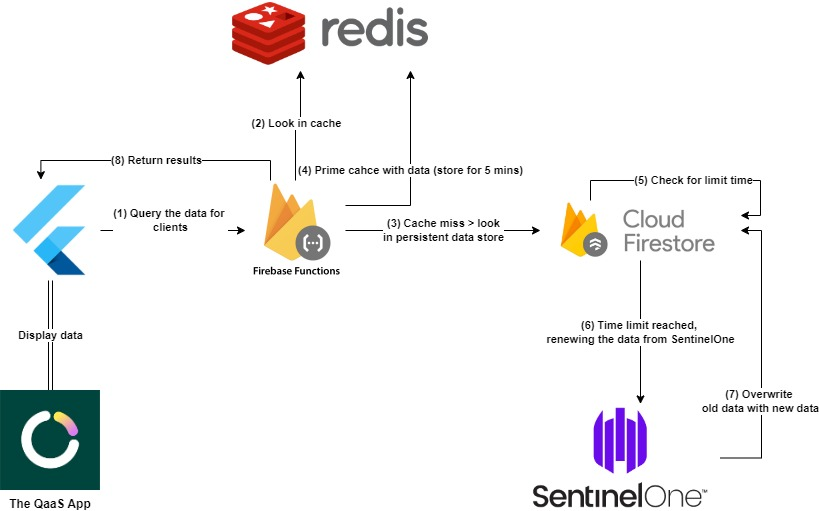
\includegraphics[width=0.9\textwidth]{Figures/Redis Caching.jpg}
  \caption{How the infrastructure would look if Redis is implemented}
\end{figure}